\chapter{Implementation}

\section{Introduction}
This chapter details the implementation of the MASDR platform. The description has been divided into software and hardware for clarity.

\section{Software Implementation}
The software for the MASDR system was written in C++ and can be found in the appendix to this report. Documentation was done with doxygen, allowing for dynamic updates to the docs whenever changes were made. The final version of the documentation can also be found in the appendix. Additionally, some python scripts were written for control patterns on the quadcopter.
\subsection{C++ vs GNU Radio}
During the design phase, there was discussion over whether to use GNU radio or C++ for the MASDR application. GNU radio would allow for more complex signal processing patterns to be constructed more easily in comparison to C++, but would increase the overhead on development and potentially at runtime as well. Using C++, the application would have to be coded entirely from scratch, interfacing with the USRP Hardware Driver (UHD) libraries, but would have much lower overhead. Based on the skills of the team members, as well as the desire for the application to be as low power and simple as possible, C++ was chosen for the application.
\subsection{Application Structure}
The MASDR Application is structured as a C++ class. The class contains methods for initialization, sampling, processing, and transmission among others. In the application’s main loop, an instance of the MASDR class updates its status and begins or changes its task based on the new status. Status is composed of both physical status, including location and heading, and software status, representing the current processing state. The processing state is an enumerated type with values SAMPLE, PROCESS, TRANSMIT, and IDLE. The state of the device determines what the processor will be doing. During operation, the application will flow from state to state as described in the state transition diagram in Figure \ref{fig:state_diagram}.
\begin{figure}[ht]
\centering
\includegraphics[width=0.70\textwidth]{img/masdr_state_diagram.png}
\caption{MASDR State Diagram}
\label{fig:state_diagram}
\end{figure}
\subsection{Sampling Procedure}
The sampling routine is mainly driven by the motion of the platform. There is a set motion pattern that the quadcopter must follow in order for the application to function correctly. At a fixed altitude, the quadcopter will travel to a sampling point and stop there. It then must rotate 360 degrees at a constant rate. After ceasing movement again, it can proceed to the next sampling point. \par
Using its own GPS receiver, the MASDR application determines whether the platform is stationary. Upon becoming stationary, the SDR begins collecting samples and the magnetometer begins logging rotation data to store with each batch of samples. Once a full rotation has been completed and the quadcopter begins moving again, the samples and rotation data are passed on to the processing routine.
\subsection{Onboard Processing}
The samples taken by the SDR are then processed to extract useful information. Given that the MASDR system is designed to be low power, a delineation between onboard processing and processing at the ground station was created. The UP board’s processor is fairly capable, allowing the initial steps of the signal processing to be done onboard. A more indepth description of the processing done onboard the MASDR platform can be found in Methodology section 5.1. The information is processed as much as possible onboard to reduce the size and duration of the transmissions to the ground station. The initial samples are also stored on a flash drive onboard so that post processing can be done on the raw data.
\subsubsection{Signal Detection Technique}
To detect the existence of a signal, an OFDM receiver in the MASDR application looks for beacon signals in the sampled data, block by block. The strength of a beacon signal is recorded with its corresponding heading, the direction the drone was facing when the block of samples were taken. This mapping is then transmitted down to the ground station for further processing.
\subsection{Data Transmission}
The MASDR platform is designed to transmit data while traveling between sampling stops after completing the processing. The transmission protocol consists of three types of messages: an idle notification, a header packet, and a data packet. The idle notification simply notifies the ground station that the MASDR platform is ready to stop and sample again. The header packet is the first packet sent after processing data; it contains a transmission ID, the location of the sampling stop, and the number of following data transmissions. The data packet consists of a transmission ID which corresponds to its header packet, a heading, and a signal strength for beacon signals at that heading.

\section{Hardware Implementation}
Using the 3DR Solo’s Development guide, the hardware for the MASDR system was developed. Combining this reference with insight into hardware implementation, the hardware was made as robust and efficient as possible.
\subsection{Mounting on Drone}
In order for the hardware to be mounted properly, the MASDR system was mounted onto the drone platform by using the Solo’s pre existing hardware mount. To do this, the 3DR Solo’s developer's guide was used to determine the dimensions of the mounting screws so that the mounting platform is able to be easily screwed onto the 3DR solo. The mounting system will connect to the bottom of the 3dr solo by using 4 M2 screws that are spaced in a 63mm x 41mm rectangular pattern as seen in Figure \ref{fig:Solo_mount}
\begin{figure}[ht]
\centering
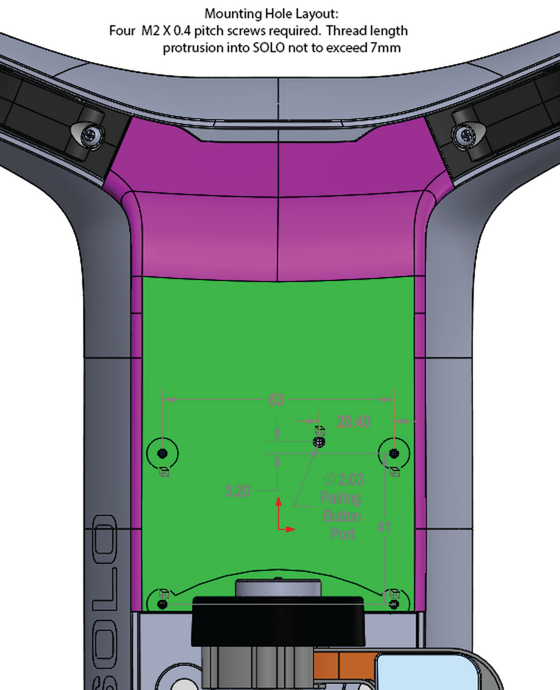
\includegraphics[width=0.70\textwidth]{img/solo_mount_points.png}
\caption{3DR Solo Mounting Points}
\label{fig:Solo_mount}
\end{figure}
\subsection{Power Conversion}
In order to ensure that the MASDR platform is powered for the entirety of the flight, we needed to ensure that we use a battery that is able to hold as much energy as possible while not adding too much weight to the drone’s payload. In addition to this, the battery must be able to support the amount of current draw that the hardware required. This became an issue for finding a suitable 5V battery that would support a constant maximum current draw of 3Amps. Instead of using a 5 Volt battery, a 12 volt battery was used, and a DC-DC converter was used to match the 5V 3A requirement. Therefore, the chosen battery was a 11.1 Volt battery which is connected to a DROK DC voltage converter so that the voltage will be converted to 5V. By down converting the voltage from the battery, we are able to draw more current from the battery than what is usually supported with a regular 5 volt battery.
\subsection{Networking Card Swap}
The 3DR solo’s default wireless card communicates to the user using the 2.4 GHz band. This interferes with sensing and locating signals on the 2.4 GHz band. In order to avoid this issue, the 2.4 GHz network card of the 3DR solo was replaced with a 5 GHz MikroTik R11e-5HnD network card instead. This ensures that the frequencies that we are sensing will be interference-free.
